%%=============================================================================
%% Methodologie
%%=============================================================================

\chapter{\IfLanguageName{dutch}{Methodologie}{Methodology}}%
\label{ch:methodologie}

%% TODO: In dit hoofstuk geef je een korte toelichting over hoe je te werk bent
%% gegaan. Verdeel je onderzoek in grote fasen, en licht in elke fase toe wat
%% de doelstelling was, welke deliverables daar uit gekomen zijn, en welke
%% onderzoeksmethoden je daarbij toegepast hebt. Verantwoord waarom je
%% op deze manier te werk gegaan bent.
%% 
%% Voorbeelden van zulke fasen zijn: literatuurstudie, opstellen van een
%% requirements-analyse, opstellen long-list (bij vergelijkende studie),
%% selectie van geschikte tools (bij vergelijkende studie, "short-list"),
%% opzetten testopstelling/PoC, uitvoeren testen en verzamelen
%% van resultaten, analyse van resultaten, ...
%%
%% !!!!! LET OP !!!!!

In dit hoofdstuk wordt de methodologie beschreven die is gebruikt om de Proof of Concept (PoC) uit te werken en te vergelijken met andere methoden voor het verkrijgen van informatie over historische en culturele locaties. Het doel van dit onderzoek is om te bepalen hoe effectief de AI-gestuurde applicatie is in vergelijking met traditionele methoden zoals het gebruik van webbronnen, fysieke verkenning en interactie met gidsen.

\section{Opzetten PoC}

\subsection{Doel}
Het hoofddoel van deze applicatie is om de ervaring van toeristen bij historische en culturele locaties te verbeteren door een interactieve, intelligente en gebruiksvriendelijke methode te bieden voor het verkrijgen van informatie over artefacten of bezienswaardigheden. Door gebruik te maken van geavanceerde kunstmatige intelligentietechnologieën, waaronder beeldherkenning en natuurlijke taalverwerking, beoogt de applicatie nauwkeurige en contextrijke informatie in realtime rechtstreeks naar het mobiele apparaat van de gebruiker te leveren.

\subsection{Systeemcomponenten}
Het systeem bestaat uit vijf hoofdcomponenten, elk met een cruciale rol binnen de algemene architectuur:

\paragraph{Android-applicatie:}
\begin{itemize}
    \item \textbf{Functionaliteit:} Dit is de gebruikersinterface waarmee toeristen met het systeem interageren. Het stelt gebruikers in staat om foto's te maken van historische artefacten of kenmerken op culturele locaties. Naast het vastleggen van afbeeldingen verzamelt de applicatie ook gebruikersvoorkeuren en feedback om de informatie te personaliseren en de gebruikersbetrokkenheid te vergroten.
    \item \textbf{Gebruikersinteractie:} De applicatie is ontworpen met een eenvoudige en intuïtieve interface, wat zorgt voor gebruiksgemak voor mensen van alle leeftijden. De belangrijkste functies omvatten een cameraknop voor het vastleggen van afbeeldingen, een geschiedenislogboek van opgevraagde items en een informatie weergavegebied waar de door ChatGPT 3.5 gegenereerde inhoud wordt gepresenteerd.
\end{itemize}

\paragraph{Java-backend:}
\begin{itemize}
    \item \textbf{Rol:} Fungeert als de middleware die gegevens van de mobiele applicatie verwerkt en communiceert met zowel de Vision API als ChatGPT 3.5. Het beheert taken zoals beeldvoorverwerking, gegevensversleuteling voor privacybescherming en API-verzoekbeheer.
    \item \textbf{Gegevensverwerking:} Na ontvangst van een afbeelding van de Android-app, voert de backend initiële gegevensverwerking uit om de afbeelding te optimaliseren voor analyse. Dit omvat het aanpassen van de grootte, het filteren en mogelijk het verbeteren van de beeldkwaliteit om de herkenningsnauwkeurigheid te verbeteren.
\end{itemize}

\paragraph{Vision API:}
\begin{itemize}
    \item \textbf{Beeldanalyse:} Maakt gebruik van machine learning-modellen om de ontvangen afbeeldingen te analyseren. Het identificeert objecten, tekst en andere relevante kenmerken binnen de afbeelding. Deze API is gekozen vanwege zijn robuustheid en hoge nauwkeurigheid bij het herkennen van diverse visuele elementen in verschillende omgevingen en lichtomstandigheden.
    \item \textbf{Data-uitvoer:} Levert gestructureerde gegevens over de herkende elementen in de afbeelding, inclusief identificatoren die kunnen worden gebruikt om via de ChatGPT 3.5 API meer gedetailleerde informatie op te halen.
\end{itemize}

\paragraph{SQL-database:}
\begin{itemize}
    \item \textbf{Dataopslag:} Bewaart alle verwerkte afbeeldingen en de bijbehorende AI-gegenereerde beschrijvingen, gebruikersgegevens, en applicatielogboeken. Dit zorgt voor persistentie van de data en maakt het mogelijk om historische gegevens te analyseren en gebruikersspecifieke aanbevelingen te doen.
    \item \textbf{Gegevensbeheer:} Verantwoordelijk voor het efficiënt beheren van gegevensqueries, updates, en verwijderoperaties. Het systeem maakt gebruik van gestructureerde querytaal om interactie met de gegevens te vergemakkelijken, wat bijdraagt aan een snelle en veilige toegang tot informatie.
    \item \textbf{Veiligheid en Privacy:} Implementeert geavanceerde beveiligingsprotocollen zoals data-encryptie en secure access controls om te zorgen dat gebruikersgegevens privé en beschermd blijven tegen ongeautoriseerde toegang.
\end{itemize}

\paragraph{ChatGPT 3.5:}
\begin{itemize}
    \item \textbf{Inhoudsgeneratie:} Ontvangt identificatoren en context van de Java-backend en genereert beschrijvende, informatieve inhoud over de geïdentificeerde objecten of scènes. Dit wordt bereikt door geavanceerde natuurlijke taalverwerkingsmodellen die mensachtige tekst kunnen genereren op basis van de invoergegevens.
    \item \textbf{Interactie:} Bovendien is het systeem ontworpen om te leren van gebruikersinteracties om de reacties te verbeteren en meer gepersonaliseerde informatie te bieden naarmate het meer wordt gebruikt.
\end{itemize}

\subsection{Gegevensstroom}

De gegevensstroom binnen het systeem is zorgvuldig ontworpen om efficiëntie en nauwkeurigheid in de verwerking en het beheer van informatie te garanderen. Hieronder volgt een gedetailleerde beschrijving van elke stap in het proces:

\subsubsection{Stap 1: Afbeelding Vastleggen}
\begin{itemize}
    \item \textbf{Gebruiker Interactie:} De gebruiker neemt een foto met de Android-applicatie. Deze foto kan een historisch artefact of kenmerk zijn binnen een culturele locatie.
    \item \textbf{Data Invoer:} De afbeelding wordt samen met eventuele extra gebruikersinput (zoals voorkeuren en feedback) opgeslagen in het tijdelijke geheugen van de applicatie.
\end{itemize}

\subsubsection{Stap 2: Data Verzending naar Backend}
\begin{itemize}
    \item \textbf{Verzending:} De afbeelding en de bijbehorende data worden via een beveiligde verbinding verzonden naar de Java-backend.
    \item \textbf{Beveiliging:} Tijdens de overdracht zijn de gegevens versleuteld om de privacy en veiligheid van de gebruikersinformatie te waarborgen.
\end{itemize}

\subsubsection{Stap 3: Voorverwerking door Backend}
\begin{itemize}
    \item \textbf{Data-ontvangen:} De Java-backend ontvangt de data en begint met de voorverwerking.
    \item \textbf{Beeldoptimalisatie:} De afbeelding wordt aangepast in grootte, gefilterd en mogelijk verbeterd om de beeldkwaliteit voor analyse te optimaliseren.
\end{itemize}

\subsubsection{Stap 4: Analyse door Vision API}
\begin{itemize}
    \item \textbf{Verzending van Afbeelding:} De geoptimaliseerde afbeelding wordt doorgestuurd naar de Vision API.
    \item \textbf{Analyse:} De Vision API gebruikt machine learning-modellen om de afbeelding te analyseren en relevante kenmerken zoals objecten en tekst te identificeren.
\end{itemize}

\subsubsection{Stap 5: Resultaten Terug naar Backend}
\begin{itemize}
    \item \textbf{Ontvangst van Data:} De Java-backend ontvangt de geanalyseerde gegevens van de Vision API, inclusief identificatoren en metadata van herkende objecten.
\end{itemize}

\subsubsection{Stap 6: Genereren van Inhoud met ChatGPT 3.5}
\begin{itemize}
    \item \textbf{Verzoek om Inhoud:} De Java-backend stuurt de identificatoren en relevante context naar ChatGPT 3.5.
    \item \textbf{Inhoudsgeneratie:} ChatGPT 3.5 genereert beschrijvende, informatieve inhoud op basis van de geïdentificeerde objecten of kenmerken.
\end{itemize}

\subsubsection{Stap 7: Opslag in SQL Database}
\begin{itemize}
    \item \textbf{Dataopslag:} De gegenereerde inhoud samen met de originele afbeelding en de analysegegevens worden opgeslagen in de SQL-database voor toekomstige referentie en analyse.
    \item \textbf{Beveiliging:} Alle opgeslagen data is beveiligd met encryptie en toegangsbeheer om te verzekeren dat alleen geautoriseerde gebruikers toegang hebben.
\end{itemize}

\subsubsection{Stap 8: Weergave aan Gebruiker}
\begin{itemize}
    \item \textbf{Terugkoppeling naar Applicatie:} De gegenereerde inhoud wordt teruggestuurd naar de Android-applicatie.
    \item \textbf{Weergave:} De gebruiker ziet de AI-gegenereerde informatie op het display van de applicatie, samen met eventuele afbeeldingen of relevante data.
\end{itemize}

\pagebreak

\subsection{Architectuurdiagram}

Hieronder wordt het architectuurdiagram gepresenteerd dat de samenhang tussen de verschillende componenten van ons systeem illustreert. De diagram toont de interacties tussen de Android-applicatie, de Java-backend, de Vision API, ChatGPT 3.5 en de SQL-database. Dit diagram is cruciaal voor het begrijpen van de gegevensstroom en de functionaliteit van elke component binnen het systeem.


\begin{figure}[ht]
    \centering
    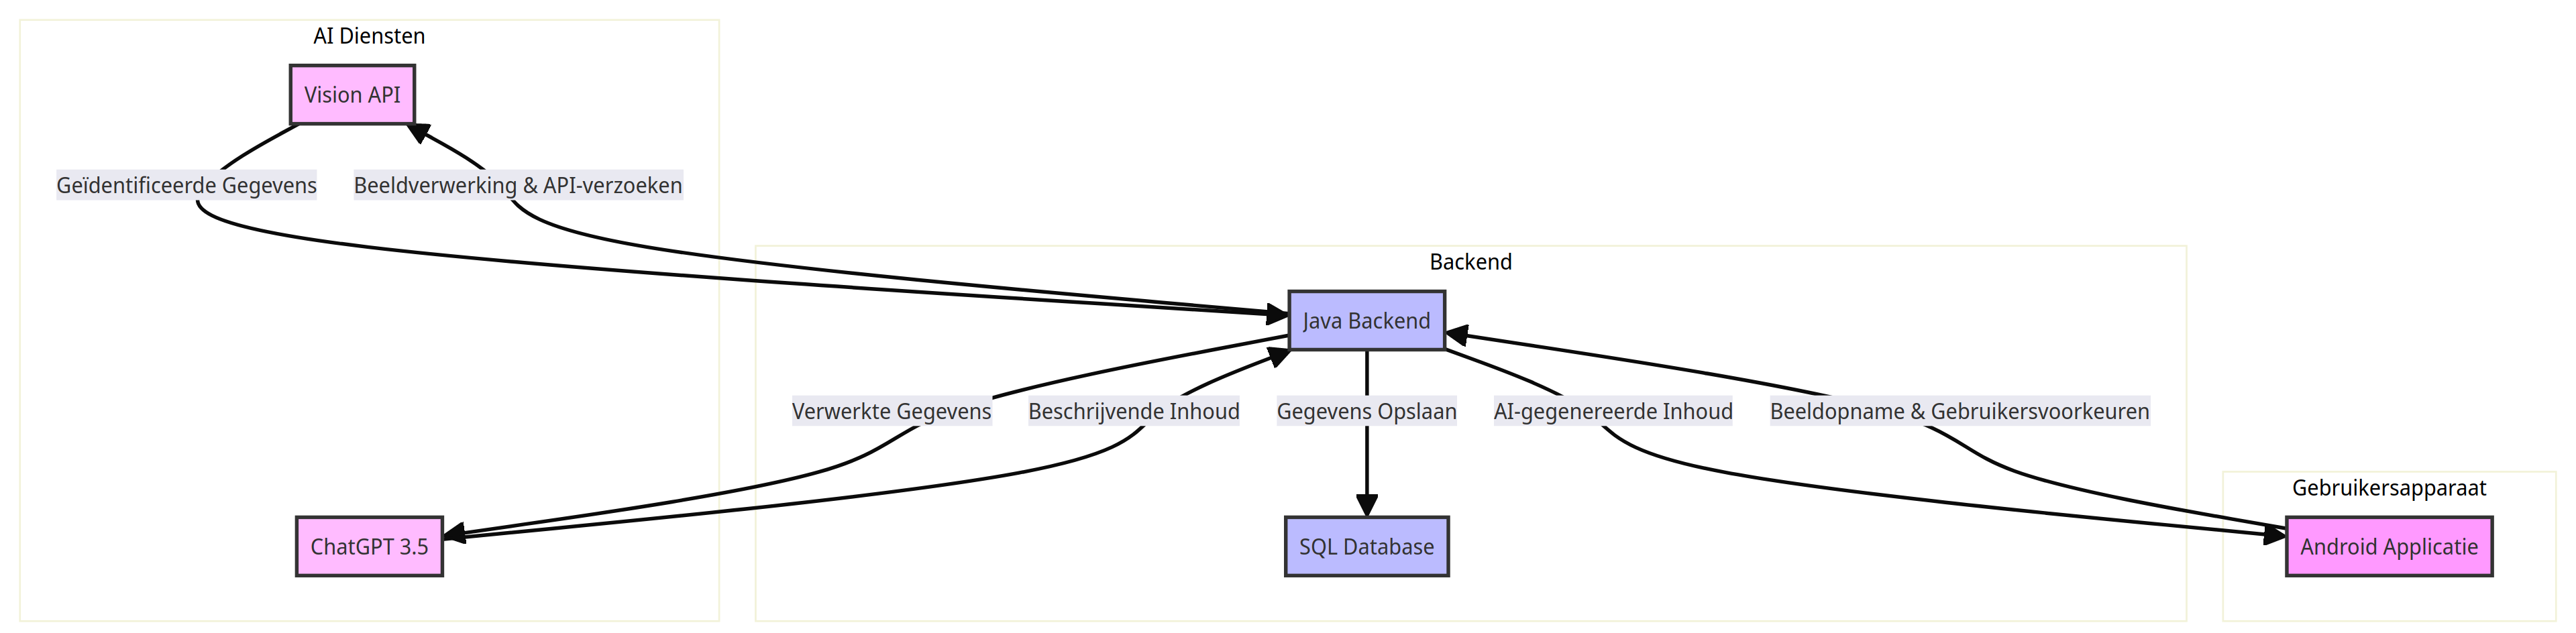
\includegraphics[width=1\linewidth]{ApplicatieArchitectuur.png}
    \caption{Architectuurdiagram}
    \label{fig:example}
\end{figure}

\section{Vergelijking met Andere Methodes}
Om de effectiviteit van de AI-gestuurde applicatie te beoordelen, wordt deze vergeleken met andere traditionele methoden om informatie te verkrijgen over historische en culturele locaties. Deze methoden omvatten het gebruik van webbronnen, fysieke verkenning ter plaatse en interactie met gidsen.

\subsection{Webbronnen}
Het gebruik van zoekmachines en online encyclopedieën zoals Google en Wikipedia is een veelgebruikte methode voor het verkrijgen van informatie. Deze methode biedt uitgebreide en gedetailleerde informatie, maar vereist tijd en inspanning om de meest relevante gegevens te vinden en te verifiëren.

\subsection{Fysieke Verkenning}
Zelfstandige fysieke verkenning van een locatie stelt bezoekers in staat om objecten en kenmerken direct te observeren. Hoewel dit een diepgaande en persoonlijke ervaring biedt, kan het ontbreken van contextuele informatie leiden tot een minder compleet begrip van de culturele en historische betekenis.

\subsection{Interacties met Gidsen}
Het gebruik van professionele gidsen biedt vaak de meest gedetailleerde en contextuele informatie. Gidsen kunnen vragen beantwoorden en aanvullende inzichten bieden die niet gemakkelijk toegankelijk zijn via andere methoden. Deze methode is echter afhankelijk van de beschikbaarheid en kwaliteit van de gids.

\subsection{Beoordelingscriteria}
De vergelijking van de verschillende methoden zal gebaseerd zijn op de volgende criteria:
\begin{itemize}
    \item \textbf{Toegankelijkheid:} Hoe gemakkelijk is het voor gebruikers om toegang te krijgen tot de informatie?
    \item \textbf{Gebruikersvriendelijkheid:} Hoe intuïtief en eenvoudig is de methode in gebruik?
    \item \textbf{Nauwkeurigheid:} Hoe nauwkeurig en betrouwbaar is de verkregen informatie?
    \item \textbf{Gebruikerstevredenheid:} Hoe tevreden zijn gebruikers met de verstrekte informatie en de algemene ervaring?
\end{itemize}

\subsection{Selectie van Testpersonen}
Voor deze vergelijkende studie zijn 14 testpersonen geselecteerd, variërend in leeftijd van 16 tot 50 jaar. Deze diversiteit in leeftijd en achtergrond zorgt voor een representatieve steekproef van de potentiële gebruikers van de applicatie. De testpersonen zijn willekeurig toegewezen aan één van de vier methoden (AI-gestuurde applicatie, webbronnen, fysieke verkenning, en interacties met gidsen) om hun ervaringen en tevredenheid te evalueren. Door deze methoden te vergelijken, wordt beoogd om te bepalen welke benadering het meest effectief is in het leveren van waardevolle en nauwkeurige informatie aan toeristen bij historische en culturele locaties.


%%
%% Het is uitdrukkelijk NIET de bedoeling dat je het grootste deel van de corpus
%% van je bachelorproef in dit hoofstuk verwerkt! Dit hoofdstuk is eerder een
%% kort overzicht van je plan van aanpak.
%%
%% Maak voor elke fase (behalve het literatuuronderzoek) een NIEUW HOOFDSTUK aan
%% en geef het een gepaste titel.

